\documentclass[14pt]{extbook}
\usepackage{multicol, enumerate, enumitem, hyperref, color, soul, setspace, parskip, fancyhdr} %General Packages
\usepackage{amssymb, amsthm, amsmath, latexsym, units, mathtools} %Math Packages
\everymath{\displaystyle} %All math in Display Style
% Packages with additional options
\usepackage[headsep=0.5cm,headheight=12pt, left=1 in,right= 1 in,top= 1 in,bottom= 1 in]{geometry}
\usepackage[usenames,dvipsnames]{xcolor}
\usepackage{dashrule}  % Package to use the command below to create lines between items
\newcommand{\litem}[1]{\item#1\hspace*{-1cm}\rule{\textwidth}{0.4pt}}
\pagestyle{fancy}
\lhead{Makeup Progress Quiz 2}
\chead{}
\rhead{Version A}
\lfoot{2790-1423}
\cfoot{}
\rfoot{Summer C 2021}
\begin{document}

\begin{enumerate}
\litem{
Choose the equation of the function graphed below.
\begin{center}
    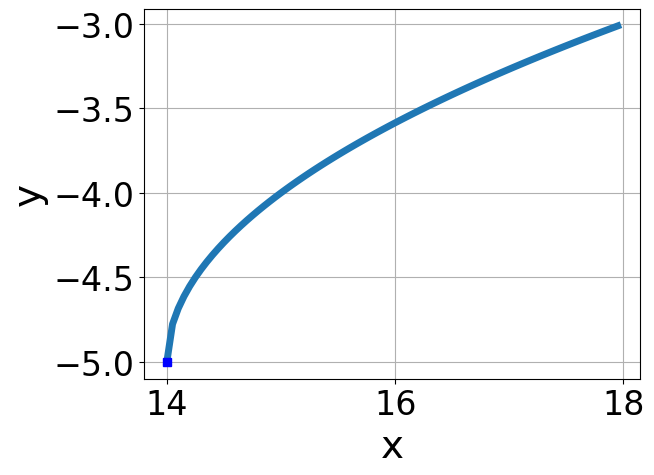
\includegraphics[width=0.5\textwidth]{../Figures/radicalGraphToEquationCopyA.png}
\end{center}
\begin{enumerate}[label=\Alph*.]
\item \( f(x) = - \sqrt{x + 14} - 5 \)
\item \( f(x) = - \sqrt{x - 14} - 5 \)
\item \( f(x) = \sqrt{x - 14} - 5 \)
\item \( f(x) = \sqrt{x + 14} - 5 \)
\item \( \text{None of the above} \)

\end{enumerate} }
\litem{
What is the domain of the function below?\[ f(x) = \sqrt[8]{9 x + 4} \]\begin{enumerate}[label=\Alph*.]
\item \( (-\infty, \infty) \)
\item \( (-\infty, a], \text{where } a \in [-7.25, -1.25] \)
\item \( (-\infty, a], \text{where } a \in [-1.44, 3.56] \)
\item \( [a, \infty), \text{ where } a \in [-0.62, 0.41] \)
\item \( [a, \infty), \text{where } a \in [-3.38, -1.86] \)

\end{enumerate} }
\litem{
Solve the radical equation below. Then, choose the interval(s) that the solution(s) belongs to.\[ \sqrt{42 x^2 + 81} - \sqrt{117 x} = 0 \]\begin{enumerate}[label=\Alph*.]
\item \( \text{All solutions lead to invalid or complex values in the equation.} \)
\item \( x_1 \in [-1.58, -1.41] \text{ and } x_2 \in [-3.9,1.3] \)
\item \( x \in [1.3,1.65] \)
\item \( x_1 \in [1.16, 1.31] \text{ and } x_2 \in [0,2.4] \)
\item \( x \in [1.16,1.31] \)

\end{enumerate} }
\litem{
Choose the graph of the equation below.\[ f(x) = - \sqrt{x + 6} + 5 \]\begin{enumerate}[label=\Alph*.]
\begin{multicols}{2}\item 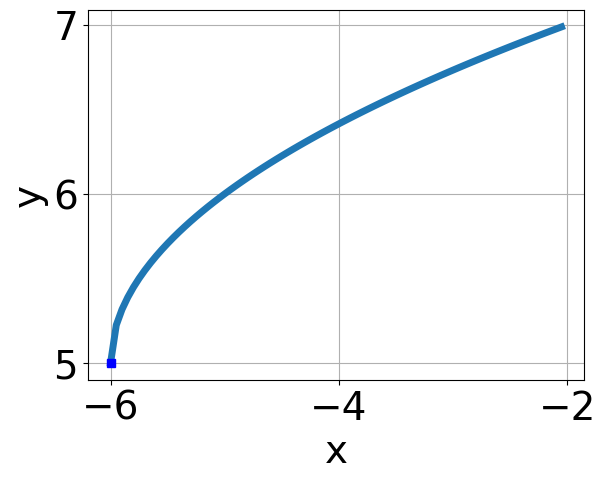
\includegraphics[width = 0.3\textwidth]{../Figures/radicalEquationToGraphAA.png}\item 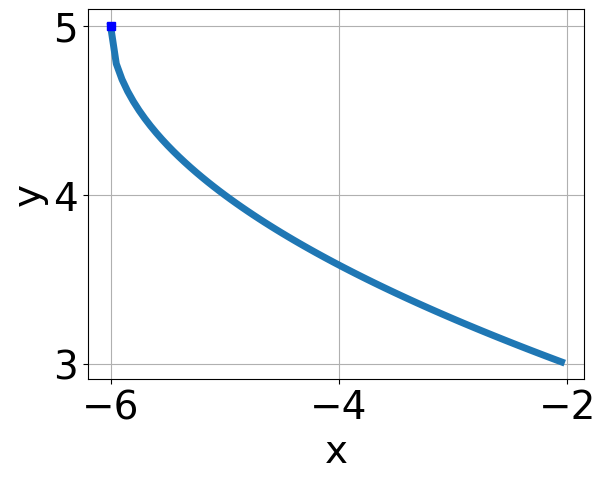
\includegraphics[width = 0.3\textwidth]{../Figures/radicalEquationToGraphBA.png}\item 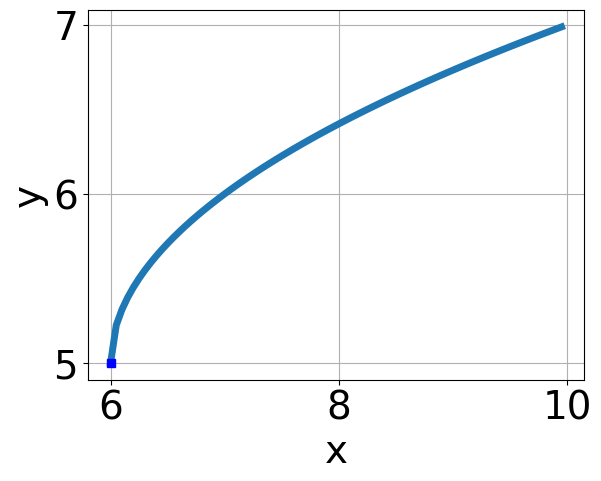
\includegraphics[width = 0.3\textwidth]{../Figures/radicalEquationToGraphCA.png}\item 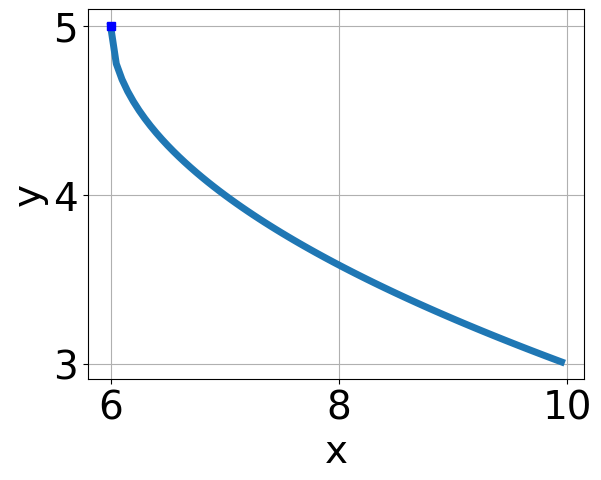
\includegraphics[width = 0.3\textwidth]{../Figures/radicalEquationToGraphDA.png}\end{multicols}\item None of the above.
\end{enumerate} }
\litem{
What is the domain of the function below?\[ f(x) = \sqrt[5]{7 x - 6} \]\begin{enumerate}[label=\Alph*.]
\item \( \text{The domain is } (-\infty, a], \text{   where } a \in [0.74, 1.13] \)
\item \( \text{The domain is } [a, \infty), \text{   where } a \in [0.58, 1.1] \)
\item \( \text{The domain is } (-\infty, a], \text{   where } a \in [1.05, 1.29] \)
\item \( \text{The domain is } [a, \infty), \text{   where } a \in [1.06, 1.55] \)
\item \( (-\infty, \infty) \)

\end{enumerate} }
\litem{
Solve the radical equation below. Then, choose the interval(s) that the solution(s) belongs to.\[ \sqrt{8 x + 3} - \sqrt{2 x - 3} = 0 \]\begin{enumerate}[label=\Alph*.]
\item \( \text{All solutions lead to invalid or complex values in the equation.} \)
\item \( x_1 \in [-0.89, -0.14] \text{ and } x_2 \in [1.5,5.5] \)
\item \( x \in [-0,0.25] \)
\item \( x \in [-1.28,-0.55] \)
\item \( x_1 \in [-1.28, -0.55] \text{ and } x_2 \in [-6.38,0.62] \)

\end{enumerate} }
\litem{
Choose the equation of the function graphed below.
\begin{center}
    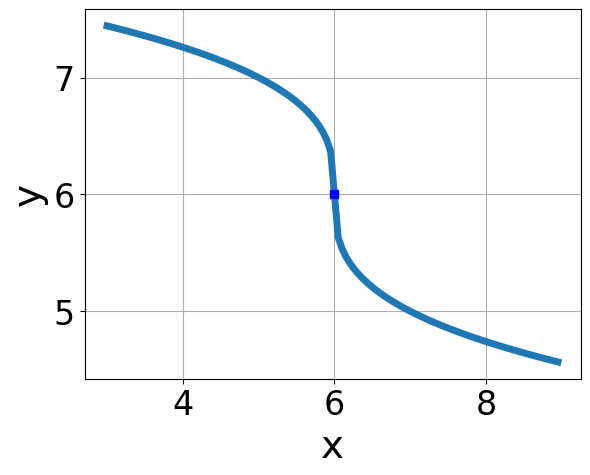
\includegraphics[width=0.5\textwidth]{../Figures/radicalGraphToEquationA.png}
\end{center}
\begin{enumerate}[label=\Alph*.]
\item \( f(x) = \sqrt[3]{x + 6} + 6 \)
\item \( f(x) = - \sqrt[3]{x - 6} + 6 \)
\item \( f(x) = \sqrt[3]{x - 6} + 6 \)
\item \( f(x) = - \sqrt[3]{x + 6} + 6 \)
\item \( \text{None of the above} \)

\end{enumerate} }
\litem{
Solve the radical equation below. Then, choose the interval(s) that the solution(s) belongs to.\[ \sqrt{-72 x^2 - 35} - \sqrt{103 x} = 0 \]\begin{enumerate}[label=\Alph*.]
\item \( x \in [-0.58,-0.54] \)
\item \( x \in [-2.23,-0.79] \)
\item \( x_1 \in [0.48, 0.89] \text{ and } x_2 \in [-0.44,8.56] \)
\item \( x_1 \in [-2.23, -0.79] \text{ and } x_2 \in [-3.56,0.44] \)
\item \( \text{All solutions lead to invalid or complex values in the equation.} \)

\end{enumerate} }
\litem{
Choose the graph of the equation below.\[ f(x) = - \sqrt[3]{x - 8} - 5 \]\begin{enumerate}[label=\Alph*.]
\begin{multicols}{2}\item 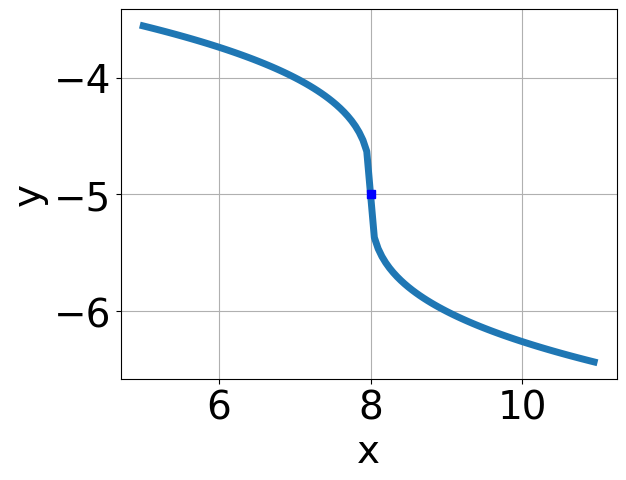
\includegraphics[width = 0.3\textwidth]{../Figures/radicalEquationToGraphCopyAA.png}\item 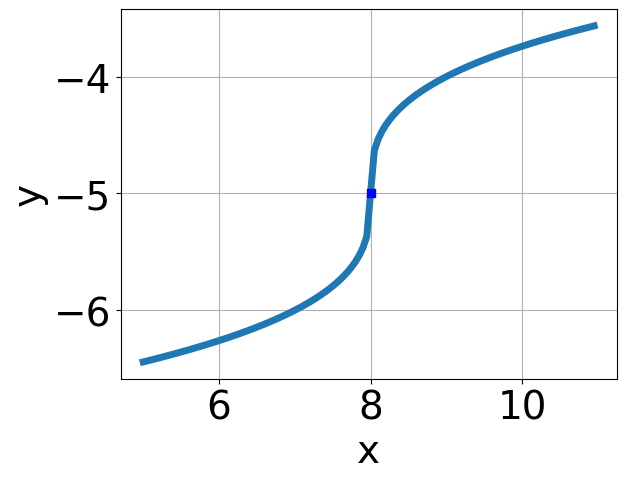
\includegraphics[width = 0.3\textwidth]{../Figures/radicalEquationToGraphCopyBA.png}\item 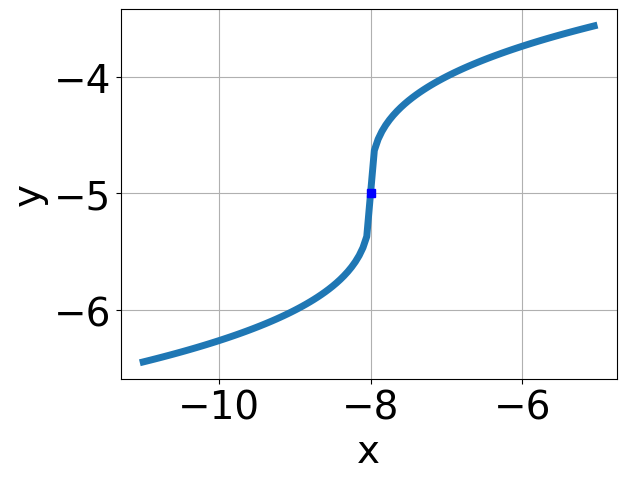
\includegraphics[width = 0.3\textwidth]{../Figures/radicalEquationToGraphCopyCA.png}\item 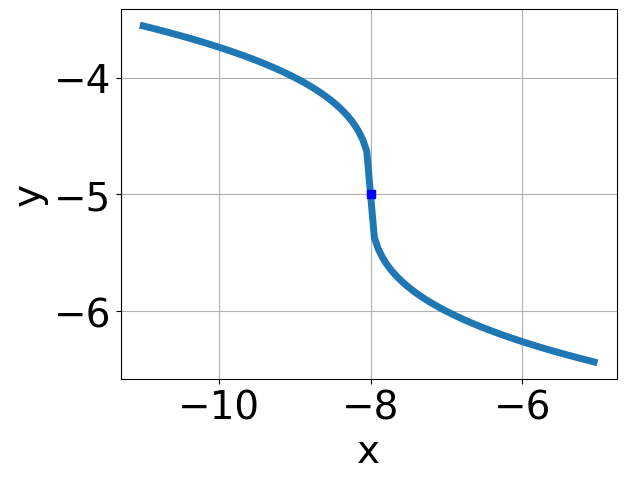
\includegraphics[width = 0.3\textwidth]{../Figures/radicalEquationToGraphCopyDA.png}\end{multicols}\item None of the above.
\end{enumerate} }
\litem{
Solve the radical equation below. Then, choose the interval(s) that the solution(s) belongs to.\[ \sqrt{-4 x + 5} - \sqrt{8 x - 3} = 0 \]\begin{enumerate}[label=\Alph*.]
\item \( x \in [0.03,0.27] \)
\item \( \text{All solutions lead to invalid or complex values in the equation.} \)
\item \( x_1 \in [0.65, 0.93] \text{ and } x_2 \in [-0.75,4.25] \)
\item \( x_1 \in [0.26, 0.42] \text{ and } x_2 \in [-0.75,4.25] \)
\item \( x \in [0.65,0.93] \)

\end{enumerate} }
\end{enumerate}

\end{document}